% This must be in the first 5 lines to tell arXiv to use pdfLaTeX, which is strongly recommended.
\pdfoutput=1
% In particular, the hyperref package requires pdfLaTeX in order to break URLs across lines.

\documentclass[11pt]{article}

% Remove the "review" option to generate the final version.
\usepackage{EACL2023}

% Standard package includes
\usepackage{times}
\usepackage{latexsym}

% For proper rendering and hyphenation of words containing Latin characters (including in bib files)
\usepackage[T1]{fontenc}
% For Vietnamese characters
% \usepackage[T5]{fontenc}
% See https://www.latex-project.org/help/documentation/encguide.pdf for other character sets

% This assumes your files are encoded as UTF8
\usepackage[utf8]{inputenc}

% This is not strictly necessary, and may be commented out.
% However, it will improve the layout of the manuscript,
% and will typically save some space.
\usepackage{microtype}

% This is also not strictly necessary, and may be commented out.
% However, it will improve the aesthetics of text in
% the typewriter font.
\usepackage{inconsolata}
\usepackage{float}
\usepackage{amsmath}


\usepackage{graphicx}
\usepackage{geometry}
\usepackage{hyperref}
\usepackage{color, soul}
\usepackage{booktabs}
% If the title and author information does not fit in the area allocated, uncomment the following
%
%\setlength\titlebox{<dim>}
%
% and set <dim> to something 5cm or larger.

\title{Analysis of Transfer Learning for Named Entity Recognition in South-Slavic Languages}

% Author information can be set in various styles:
% For several authors from the same institution:
% \author{Author 1 \and ... \and Author n \\
%         Address line \\ ... \\ Address line}
% if the names do not fit well on one line use
%         Author 1 \\ {\bf Author 2} \\ ... \\ {\bf Author n} \\
% For authors from different institutions:
% \author{Author 1 \\ Address line \\  ... \\ Address line
%         \And  ... \And
%         Author n \\ Address line \\ ... \\ Address line}
% To start a seperate ``row'' of authors use \AND, as in
% \author{Author 1 \\ Address line \\  ... \\ Address line
%         \AND
%         Author 2 \\ Address line \\ ... \\ Address line \And
%         Author 3 \\ Address line \\ ... \\ Address line}


\author{Nikola Ivačič $^{1}$\\{\bf Hanh Thi Hong Tran$^{1,2,3}$}\\ {\bf Boshko Koloski$^{1,2}$} \\ {\bf Senja Pollak$^{1}$}\\
$^1$Jožef Stefan Institute,\\ $^2$Jožef Stefan IPS, \\ 1000 Ljubljana, Slovenia \\
\And
 \textbf{Matthew Purver$^{1,4}$} \\  
$^3$ University of La Rochelle \\17000 La Rochelle,  France \\
$^4$School of Electronic Engineering\\ and Computer Science\\Queen Mary University of London\\ London E1 4NS, UK
}

\begin{document}
\maketitle

\begin{abstract}
This paper focuses on Named Entity Recognition for South-Slavic languages using pre-trained multilingual neural network models.
We investigate whether the performance of the models for a target language can be improved by using data from closely related languages.
The results show that this is not the case for the Slovene language, while for Croatian and Serbian, the results are better in selected cross-lingual settings.
The most significant performance improvement is observed for the Serbian language, which has the smallest corpora, showing the potential of the method in less-resourced settings.
\end{abstract}


\section{Introduction}
\label{sec:introduction}

Named Entity Recognition (NER) is one of the cornerstones of the NLP tasks and is widely used in many real-life applications, including in the news industry.
In our study, we focus on South-Slavic languages and investigate whether the performance of the models for a target language can be improved by using data from closely related languages.

The research on NER has a long history. Already in the 90s, the research was performed by \citet{grishman1996message}, followed by \citet{sang2003introduction,segura2013semeval}, to mention a few of the early works. 
Early literature focused on rule-based models \cite{yu2020named}, which were based on a set of pre-defined patterns, and hand-crafted rules (e.g., LTG, NetOwl). 
These approaches were followed by the unsupervised methods \cite{collins1999unsupervised,nadeau2006unsupervised}, where no annotated data were required. 
The advent of machine learning algorithms opened a novel direction for NER tasks where feature engineering gained more traction \cite{krishnan2006effective,mansouri2008named,liu2020hamner}. 
With recent advances in neural networks, NER was formulated as a sequence-labelling task and took advantage of the neural systems, especially Transformers, to minimize the effort of feature engineering \cite{lample2016neural,hanh2021named}. 
Ensemble systems that combine different machine learning \cite{ekbal2011weighted,saha2013combining} and neural representation \cite{hanh2021named} or architectures \cite{chiu2016named,liu2018empower} were also under consideration. 
Besides rich-resourced languages (e.g., English), there is a shift to several less-resourced ones, including the Slavic family (see several organized shared tasks \citet{piskorski-etal-2017-first,piskorski-etal-2019-second,piskorski-etal-2021-slav}).

The availability of multilingual large language models and transfer learning strategies \cite{devlin-etal-2019-bert} have simplified the cross-lingual transfer for a variety of NLP tasks. 
This opened new opportunities in the development of multilingual applications, especially in settings with limited resources. 
Cross-lingual learning allows for overcoming the problems with the lack of data, including in zero- and few-shot learning, where no or very small number of data for the target language is available.
Moreover, getting the performance of a multilingual neural model as close as possible to the performance of a monolingual one can be very beneficial also in terms of simplicity and scalability, as a single model can be used instead of many monolingual ones. Last but not least, even if data for the target language is available, adding data in other languages can lead to an improvement in results.

Multilingual models have been used in a large number of tasks, including cross-lingual hate-speech detection \cite{Pelicon2021peerj}, zero-shot sentiment analysis \cite{pelicon-etal-2021-zero} as well as for NER \cite{arkhipov2019tuning,suppa2021benchmarking}.
It was shown that the multilingual BERT transformer model outperforms the BiLSTM-CRF model for the NER task. 
The performance can be even further improved with a word-level CRF layer \cite{arkhipov2019tuning}. 
Nevertheless, it is also evident that XLM-Roberta outperforms BERT \cite{suppa2021benchmarking} in such tasks. 
The closest to our paper is the work by ~\citet{prelevikj-zitnik-2021-multilingual}, who showed that the monolingual NER model performance for the Slovene language is practically equal to that of a multilingual one.

In our paper, we focus on NER in Slovene, Croatian and Serbian and aim to answer the following question: does fine-tuning with related languages influence the performance of a multilingual model compared to fine-tuning only in the target language?

The rest of the paper is structured as follows. 
First, we present the corpora we used and how we preprocessed them, followed by their analysis.
Next, we continue with presenting the methodology, where we first introduce the measures, models, hyper-parameters, and software used.
Finally, we continue by evaluating the results and by presenting conclusions.

\section{Data Description}
\label{sec:data-description}
In this section, we first present all the corpora used. Then, we continue with the description of the conversion of these datasets to the expected format and conclude with the corpora structure analysis.

We used the most common and established NER corpora for selected languages (see Table~\ref{tab:corpora}).
The assumption and strategy for gathering corpora were also: ``the more, the better.''
\begin{table}
  \caption{List of Used Corpora, which shows each corpus with an abbreviated name used in this paper, followed by the number of sentences, the number of tokens it contains, and lastly, its long name.}
  \label{tab:corpora}
  \resizebox{\linewidth}{!}{\begin{tabular}{lrrl}
    \toprule
    Corpus&Sentences&Tokens&Long Name\\
    \midrule 
    \multicolumn{4}{c}{Slovene} \\
    \midrule
    bsnlp&18106&400291&BSNLP 2017/21~\cite{piskorski-etal-2021-slav}\\
    500k&9483&193611&ssj500k 2.3~\cite{ssj500k-23}\\
    ewsd&2024&31233&{ELEXIS}-{WSD} 1.0~\cite{ELEXIS-WSD-10}\\
    scr&18139&391526&{SentiCoref} 1.0~\cite{SentiCoref-10}\\
    \midrule
    \multicolumn{4}{c}{Croatian} \\
    \midrule
    bsnlp&820&18704&BSNLP 2017 and 2021~\cite{piskorski-etal-2021-slav}\\
    500k&24780&504227&hr500k 1.0 ~ \cite{hr500k-10}\\
    \midrule
    \multicolumn{4}{c}{Serbian} \\
    \midrule
    set&3891&86726&{SETimes}.{SR} 1.0~\cite{SETimes-SR-1.0}\\
    \midrule    
    \multicolumn{4}{c}{Bosnian} \\
    \midrule
    wann&8917&199378&WikiANN / PAN-X~\cite{rahimi-etal-2019-massively}\\
    \midrule    
    \multicolumn{4}{c}{Macedonian} \\
    \midrule
    wann&16227&156467&WikiANN / PAN-X~\cite{rahimi-etal-2019-massively}\\
  \bottomrule
  \end{tabular}}
\end{table}

We used NER tags in IOB2~\cite{IOB2} format from the CoNLL-2003 shared task~\cite{CoNLL2003} as a common denominator for all corpora and experiments.
Each corpus was first combined if split, then converted to a common format, reshuffled, and split to train/validation/test set in an 80/10/10 ratio.

We produced combined corpora by concatenating the sets without further reshuffling so that the experiments could be repeated.

Our study uses Slovene, Croatian, and Serbian as target languages. However, in addition to those, also Bosnian and Macedonian are considered as the source languages, as they are closely related.

Corpora used are presented in Table~\ref{tab:corpora}. 
Note that the ones for Slovene were obtained from BSNLP and parts of a newly published combined Training corpus {SUK} 1.0~\cite{SUK-1.0}, which contained NER annotations (ssj500k, ELEXIS-WSD, and SentiCoref). 

%\hl{Ni jasno, zakaj tukaj samo za slovenscino opises. Zakaj ta korpus ne nastopa v tabeli? Skratka, prej trdis, da uporabis korpuse iz tabele 1, tukaj nekaj drugega. V tabeli 1 jasno opisi, kaj uporabis, pa potem das lahko ta stavek ven. }

\subsection{Data Conversion}
\label{subsec:data-conversion}
The first obstacle was the different NER tags used in corpora.
We decided to keep only the common tags: PER, LOC, and ORG\@.
For example, the BSNLP corpus uses PRO and EVT tags, while the \textit{wann} corpus lacks a MISC tag common to 500k training corpora.
All non-common tags, including MISC, were replaced with O (outside IOB).

The second obstacle was the difference in format.
BSNLP corpus, for instance, uses separate files for verbatim text and NER tags, with no positional reference between one another. We used CLASSLA~\cite{ljubesic-dobrovoljc-2019-neural} sentence segmentation and tokenization with a custom conversion script to solve this problem. 

In addition, we removed a small amount (54) of very short sentences, as they were often noisy (e.g. conversion errors).

Next, we converted corpora from standard CoNLL format to CSV format with two fields:
\begin{itemize}
  \item Sentence: whitespace separated sentence word tokens.
  \item NER: white space separated NER tags for each sentence word token.
\end{itemize}

\begin{table}[H]
  \caption{Example whitespace separated sentence word tokens with corresponding IOB2 NER tags.}
  \label{tab:ner_example}
  \resizebox{\linewidth}{!}{\begin{tabular}{llllll}
    \toprule
    Obtoženka&Asia&Bibi&zapustila&Pakistan\\
    \midrule
    O&B-PER&I-PER&O&B-LOC\\
    \bottomrule
  \end{tabular}}
\end{table}
Finally, we split the corpus data into train, validation, and test sets.

\subsection{Corpora analysis}
\label{subsec:corpora-analysis}
Comparing the corpora showed the differences that could potentially be problematic for obtaining aligned model performance.
Especially considering the NER tag ratios where the WikiANN automatically annotated corpora structure was standing out (see Table~\ref{tab:corpora_analysis} and Figure~\ref{fig:corpora_analysis}). 
This is also one of the reasons why in our experiments, WikiANN corpora were only considered for additional training but not as target language gold standards.

\begin{table}[H]
  \caption{Analysis of Combined Corpora - shows each language's combined corpora number of tokens per sentence, followed by the number of NER tags per token. 
  Finally, the PER, LOC, and ORG columns show the ratios with respect to all NER tags.}
  \label{tab:corpora_analysis}
  \resizebox{\linewidth}{!}{\begin{tabular}{lrrrrr}
    \toprule
    Lang.&tok./sent.&NER/tok.&PER\%&LOC \%&ORG \%\\
    \midrule
    sl&21.29&9.09\%&31.70\%&22.20\%&34.13\%\\
    hr&20.43&7.41\%&28.71\%&20.55\%&30.82\%\\
    sr&22.29&12.01\%&29.96\%&30.12\%&32.35\%\\
    bs&\textbf{7.81}&\textbf{36.91\%}&31.65\%&29.67\%&38.67\%\\
    mk&\textbf{9.64}&\textbf{28.07\%}&34.89\%&30.32\%&34.79\%\\
    \bottomrule
  \end{tabular}}
\end{table}

\begin{figure}[h]
  \centering
  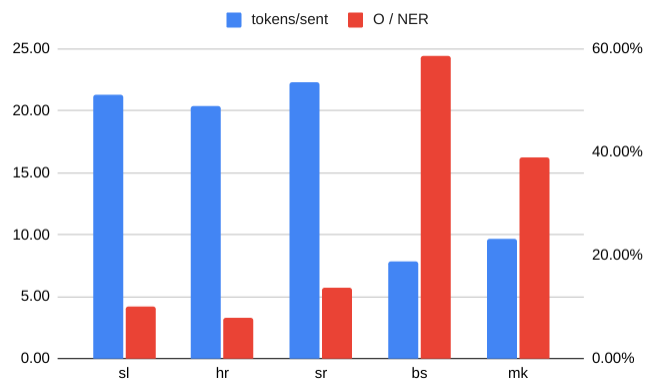
\includegraphics[width=\linewidth]{wikiann-skew}
  \caption{WikiANN corpus skew}
  \label{fig:corpora_analysis}
\end{figure}

Fortunately, we were unable to detect any inconsistencies regarding performance measurements.

\section{Methodology}
\label{sec:methods}
In the following section, we present the methodology used in our experiments to test our hypothesis that
the NER classification F1-score increases when we fine-tune the pre-trained multilingual model with an additional, related language.

\subsection{Method}
\label{subsec:method}
The selected method was first to select the pre-trained embeddings, train the baseline model for each language and produce NER classification measurements.
Baseline models were fine-tuned with only one - target language.

We experimented with two multilingual models, BERT multilingual base model (cased)~\cite{DBLP:journals/corr/abs-1810-04805} and XLM-RoBERTa (base-sized model)~\cite{DBLP:journals/corr/abs-1911-02116}.
However, pilot results showed better performance of XLM-RoBERTa, which was used in the final experiments presented in this paper.

Next, we combined additional language corpora, re-trained the model, and measured performance on the target language test set again.
We focus only on three selected languages for evaluation, Slovene, Croatian and Serbian, but consider Bosnian and Macedonian as additional source languages.

We used the HuggingFace transformers Python library~\cite{wolf-etal-2020-transformers} for all the experiments.

\subsection{Parameters}
\label{subsec:parameters}
For all the experiments, we used the following hyper-parameters:
\begin{itemize}
  \item 256 max-length for tokenizer
  \item PyTorch's AdamW algorithm with 5e-5 learning rate
  \item batch size of 20
  \item 40 epochs (preliminary runs showed  best F1-scores between epochs 15 and 35)
  \item F1-score for best model selection and training progression.
\end{itemize}

\section{Evaluation}
\label{sec:evaluation}
In the following section, we define the F1-score we used for evaluation. 
Then we present the experiment results: the evaluation of the pre-trained multilingual model, followed by the evaluation of fine-tuning for each language.

For all classification measurements, the Seqeval library~\cite{seqeval} was used.
Although the library uses CoNLL evaluation by default, we chose ``strict'' mode evaluation.
When calculating measurements, the strict mode also considers the IOB2 tag's ``beginning'' and ``inside'' parts.
Therefore the NER tags must match exactly.

\subsection{Evaluation measure}
For the evaluation of the classification models, we used the traditional F-measure or balanced F-score, which is the harmonic mean of precision and recall:
\begin{equation*}
    \text{F1-score} = 2  \cdot \frac{Precision \cdot Recall}{Precision +  Recall}
\end{equation*}
The Precision and Recall are defined as:
\begin{equation*}
\begin{split}
    \text{Precision} = \frac{TP}{TP + FP}
\end{split}
\quad\quad
\begin{split}
    \text{Recall} = \frac{TP}{TP + FN}
\end{split}
\end{equation*}
given that:
\begin{itemize}
  \item FP: a NER tag that is predicted but not present in the test.
  \item FN: a NER tag present in the test but missing in our prediction.
  \item TP: a NER tag that is correctly predicted.
\end{itemize}

The overall F1-score, used in the evaluation tables and figures, is a macro-averaged F1-score over all three NER tags. 
Macro-averaged F1-score is computed using the arithmetic mean of all the per-class F1 scores:
\begin{equation*}
    \text{Macro-averaged F1-score} = \frac{1}{n}\sum_{i=1}^{n} F1_i
\end{equation*}
where $F1_i$ is the F1-score for $ith$ NER tag.

The average distance from the baseline was used as a measure to show the overall variability of different models tested with the same test set. We also report the maximum reduction in error rate achieved for each tag.

\subsection{Results}
Here, we present results for the three target languages.
\subsubsection{Slovene}
\label{subsec:slovene}

\begin{figure}[H]
  \centering
  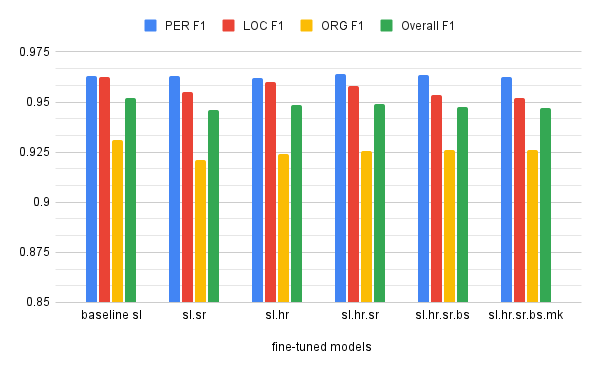
\includegraphics[width=\linewidth]{eval_sl}
  \caption{Slovene language test set model performance} %\hl{Sorting the bars in a barchart with respect of the dataset is not much informative - since we are visually asked to compare same colored bars that will always be spatially distant from one another. Consider grouping the bars by the metric rather than the dataset. }}
  \label{fig:eval_sl}
\end{figure}

The Slovene test set shows surprising model stability.
This stability comes, assumingly, from larger corpora compared to the others.
It might be that the quality of the corpora also plays a crucial role in this observation.

\begin{table}[H]
  \caption{Slovene language test set model performance}
  \label{tab:eval_sl}
  \resizebox{\linewidth}{!}{\begin{tabular}{lrrrrr}
    \toprule
    Model&PER F1&LOC F1&ORG F1&Overall F1\\
    \midrule
    baseline sl&0.963&\textbf{0.963}&\textbf{0.931}&\textbf{0.952}\\
    \midrule
    sl.sr&0.963&0.955&0.921&0.946\\
    sl.hr&0.962&0.960&0.924&0.948\\
    sl.hr.sr&\textbf{0.964}&0.958&0.925&0.949\\
    sl.hr.sr.bs&\textbf{0.964}&0.953&0.926&0.948\\
    sl.hr.sr.bs.mk&0.962&0.952&0.926&0.947\\
    \midrule
%    avg.\ dist.&0.00071&0.00695&0.00634&0.00433\\
    avg.\ dist.&0.00071&0.0070&0.0063&0.0043\\
    error reduction & 2.7\% & - & - & - \\
    \bottomrule
  \end{tabular}}
\end{table}

If we observe the average distance from the baseline in the table's last row, we can see that it is only near 0.5\%. For the PER tag, the error rate is reduced by a small amount (2.7\%), but other tags are not improved.

\subsubsection{Croatian}
\label{subsec:croatian}

The Croatian language test set shows higher  variability when tested with different models, most significantly on the ORG tag.
It might be that the other corpora training is influencing variability.
However, there is now some overall performance gain from the training: we can see that the average distance from the baseline is 0.5-1\%, with reductions in error rates between 6 and 11\%.
\begin{figure}[h]
  \centering
  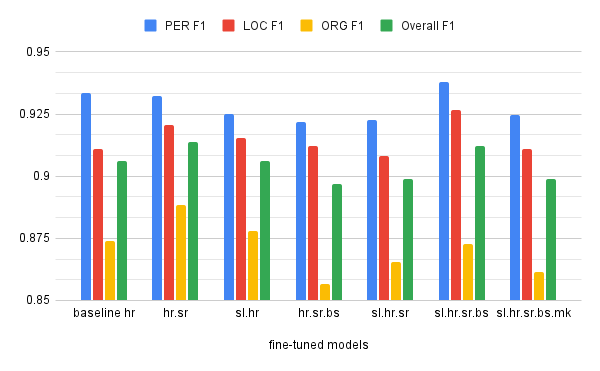
\includegraphics[width=\linewidth]{eval_hr}
  \caption{Croatian language test set model performance}
  \label{fig:eval_hr}
\end{figure}

\begin{table}[H]
  \caption{Croatian language test set model performance}
  \label{tab:eval_hr}
  \resizebox{\linewidth}{!}{\begin{tabular}{llrrrr}
    \toprule
    Model&PER F1&LOC F1&ORG F1&Overall F1\\
    \midrule
    baseline hr&0.934&0.911&0.874&0.906\\
    \midrule
    hr.sr&0.932&0.921&\textbf{0.888}&\textbf{0.914}\\
    sl.hr&0.925&0.915&0.878&0.906\\
    hr.sr.bs&0.922&0.912&0.856&0.897\\
    sl.hr.sr&0.923&0.908&0.865&0.899\\
    sl.hr.sr.bs&\textbf{0.938}&\textbf{0.927}&0.873&0.912\\
    sl.hr.sr.bs.mk&0.925&0.911&0.861&0.899\\
    \midrule
%    avg.\ dist.&0.00757&0.00554&0.00977&0.00624\\
    avg.\ dist.&0.0076&0.0055&0.0098&0.0062\\
    error reduction & 6.1\% & 18.0\% & 11.1\% & 8.5\% \\
    \bottomrule
  \end{tabular}}
\end{table}

\subsubsection{Serbian}
\label{subsec:serbian}
The Serbian language test set showed the most significant increase in performance over the baseline.
Its average distance in performance measurements from the baseline is from approximately 0.5\% to 2.5\%, with large reductions in error rate of 43\%-68\%.
The main suspect for this phenomenon is the Serbian corpus size. %\hl{this is an interesting insight, would you dare to draw a plot (or ranking) of the F1-Score divided by the LOGARITHM of the number of training instances per language, maybe we can support this claim strongly) }
It is the smallest included in this analysis, and therefore benefits most from additional cross-lingual training on other corpora. % and the most easily influenced by other corpora.
\begin{figure}[h]
  \centering
  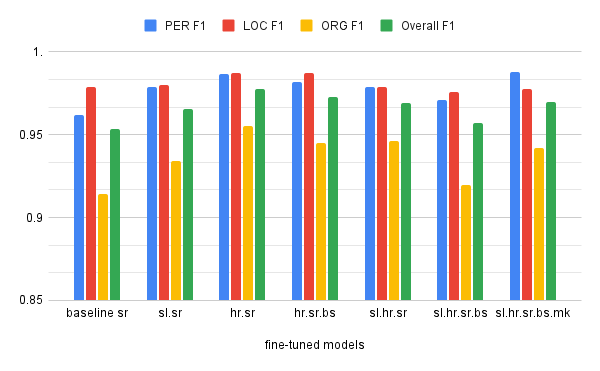
\includegraphics[width=\linewidth]{eval_sr}
  \caption{Serbian language test set model performance}
  \label{fig:eval_sr}
\end{figure}

\begin{table}[H]
  \caption{Serbian language test set model performance}
  \label{tab:eval_sr}
  \resizebox{\linewidth}{!}{\begin{tabular}{llrrrr}
    \toprule
    Model&PER F1&LOC F1&ORG F1&Overall F1\\
    \midrule
    baseline sr&0.962&0.979&0.914&0.954\\
    \midrule
    sl.sr&0.979&0.980&0.934&0.965\\
    hr.sr&0.987&\textbf{0.988}&\textbf{0.956}&\textbf{0.978}\\
    hr.sr.bs&0.982&0.987&0.945&0.973\\
    sl.hr.sr&0.979&0.979&0.946&0.969\\
    sl.hr.sr.bs&0.971&0.976&0.920&0.957\\
    sl.hr.sr.bs.mk&\textbf{0.988}&0.978&0.942&0.970\\
    \midrule
    %avg.\ dist.&0.01885&0.00372&0.02603&0.01504\\
    avg.\ dist.&0.019&0.0037&0.026&0.015\\
    error reduction & 68.4\% & 42.9\% & 48.8\% & 52.2\%\\
    \bottomrule
  \end{tabular}}
\end{table}

\section{Conclusion}
\label{sec:conclusion}
We have shown that model performance can be influenced substantially by cross-lingual training with other language corpora, but that improvements only seem to occur if the target language has relatively small corpora. 
While for Slovene, the monolingual setting generally performs better, for Croatian and Serbian, the results are slightly better in selected cross-lingual settings.
The most significant performance improvement is shown for the Serbian language, which has the smallest corpora. 
This indicates that fine-tuning with other closely related languages may benefit only the ``low resource'' languages.

Our initial hypothesis has not been fully upheld, but the result is still beneficial. 
First, when considering less-resourced settings, leveraging closely related languages is beneficial. 
Second, the performance does not degrade much if we fine-tune the model with additional language corpora from the same family.
This is an important finding, as using a multilingual model in an application is a simpler solution than having several monolingual models.

In future work, we propose further investigating how performance changes when distantly related languages are used for fine-tuning the models. 
This will further benefit the usage in an industrial setting if the performance is not degraded, as having a single model that supports more languages with similar performance to monolingual training is more scalable and practical.

\section*{Acknowledgements}

We acknowledge financial support from several sources: the Slovenian Research Agency via research core funding for the programme Knowledge Technologies (P2-0103) and the projects CANDAS (Computer-assisted multilingual news discourse analysis with contextual embeddings, J6-2581) and SOVRAG (Hate speech in contemporary conceptualizations of nationalism, racism, gender and migration, J5-3102); the UK EPSRC via the projects Sodestream (Streamlining Social Decision Making for Improved Internet Standards, EP/S033564/1) and ARCIDUCA (Annotating Reference and Coreference In Dialogue Using Conversational Agents in games, EP/W001632/1); and via the project RobaCOFI (Robust and adaptable comment filtering), which indirectly received funding from the European Union's Horizon 2020 research and innovation action programme via the AI4Media Open Call \#1 issued and executed under the AI4Media project (Grant Agreement no.\ 951911).  This paper reflects only the authors' views; the EC and the AI4Media project are not responsible for any use that may be made of the information contained herein.

\bibliography{anthology,custom}
\bibliographystyle{acl_natbib}


\end{document}
